\chapter{KINEMATIC PROBLEM}

\section{Topic}
Formulate the forward kinematic problem. Then determine the coordinates of the end-point 
according to the three joint variables. Make a plot for a certain case.
 
\section{Theory}

The transformaytion matrix $^{i-1}_{i}T$ to transform coordinate frames \textbf{$B_i$} to \textbf{$B_i - 1$} is represented as a product of four basic transformations using paramaters of link $(i)$ and joint $i$

\begin{align}
^{i-1}_{i}T = 
\begin{bmatrix}
\cos(\theta_i) & -\sin(\theta_i)\cos(\alpha_i) & \sin(\theta_i)\sin(\alpha_i) & a_i\cos(\theta_i) \\
\sin(\theta_i) & \cos(\theta_i)\cos(\alpha_i) & -\cos(\theta_i)\sin(\alpha_i) & a_i\sin(\theta_i) \\
0 & \sin(\alpha_i) & \cos(\alpha_i) & d_i \\
0 & 0 & 0 & 1
\end{bmatrix}
\end{align}

To find the single transformation that relates frame \{$i$\} to frame \{0\}, the transformation matrices of every link are then multiplied together:

\begin{equation}
^{0}_{i}T = ^{0}_{1}T \ ^{1}_{2}T\ ... \ ^{i-1}_{i}T
\end{equation}

This transformation $^{0}_{i}T$ is a function of all $i$ joint variables. If the robot's joint-position sensors are queried, the Cartesian position and orientation of the end effector could be computed by $^{0}_{i}T$.



\section{Application}
We have:

\begin{equation}
    ^{0}T_{1} = 
    \begin{bmatrix}
    \cos\theta_1 & -\sin\theta_1 & 0 & 0 \\
    \sin\theta_1 & \cos\theta_1 & 0 & 0 \\
    0 & 0 & 1 & 0 \\
    0 & 0 & 0 & 1
    \end{bmatrix}
\end{equation}

\begin{equation}
    ^{1}T_{2} = 
    \begin{bmatrix}
    1 & 0 & 0 & 0 \\
    0 & 1 & 0 & 0 \\
    0 & 0 & 1 & d_2 \\
    0 & 0 & 0 & 1
    \end{bmatrix}
\end{equation}

\begin{equation}
    ^{2}T_{3} = 
    \begin{bmatrix}
    1 & 0 & 0 & \ell_3 \\
    0 & 1 & 0 & 0 \\
    0 & 0 & 1 & 0 \\
    0 & 0 & 0 & 1
    \end{bmatrix}
\end{equation}

\begin{equation}
    ^{3}T_{4} = 
    \begin{bmatrix}
    \cos\theta_4 & -\sin\theta_4 & 0 & \ell_4\cdot\cos\theta_4 \\
    \sin\theta_4 & \cos\theta_4 & 0 & \ell_4\cdot\sin\theta_4 \\
    0 & 0 & 1 & 0 \\
    0 & 0 & 0 & 1
    \end{bmatrix}
\end{equation}

Thus

\begin{equation*}
    ^{0}T_{4} = ^{0}T_{1}.^{1}T_{2}.^{2}T_{3}.^{3}T_{4}
    = 
    \begin{bmatrix}
    \cos(\theta_1 + \theta_4) & -\sin(\theta_1 + \theta_4) & 0 & \ell_4.\cos(\theta_1 + \theta_4) + \ell_3.\cos\theta_1 \\
    \sin(\theta_1 + \theta_4) & \cos(\theta_1 + \theta_4) & 0 & \ell_4.\sin(\theta_1 + \theta_4) + \ell_3.\sin\theta_1 \\
    0 & 0 & 1 & d_2 \\
    0 & 0 & 0 & 1
    \end{bmatrix}
\end{equation*}

In conclusion, we have the solution for the forward kinematic problem as below


\begin{equation}
    \begin{bmatrix}
        x  \\
        y \\
        z 
        \end{bmatrix}
    = 
    \begin{bmatrix}
        \ell_4.\cos(\theta_1 + \theta_4) + \ell_3.\cos\theta_1 \\
        \ell_4.\sin(\theta_1 + \theta_4) + \ell_3.\sin\theta_1 \\
        d_2 
        \end{bmatrix}
\end{equation}

Make a plot for a certain case: \\
\hspace*{0.6cm} During the time \( t \) from 0s to 10s, the input \( (\theta_1, d_2, \theta_4) \) gradually increases from \( (0^\circ, 2200, 0^\circ) \) to \( (90^\circ, 2700, 90^\circ) \). Using MATLAB, the position \( (x, y, z \) of the end-effector can be plotted as below:
\begin{figure}[H]
    \centering
    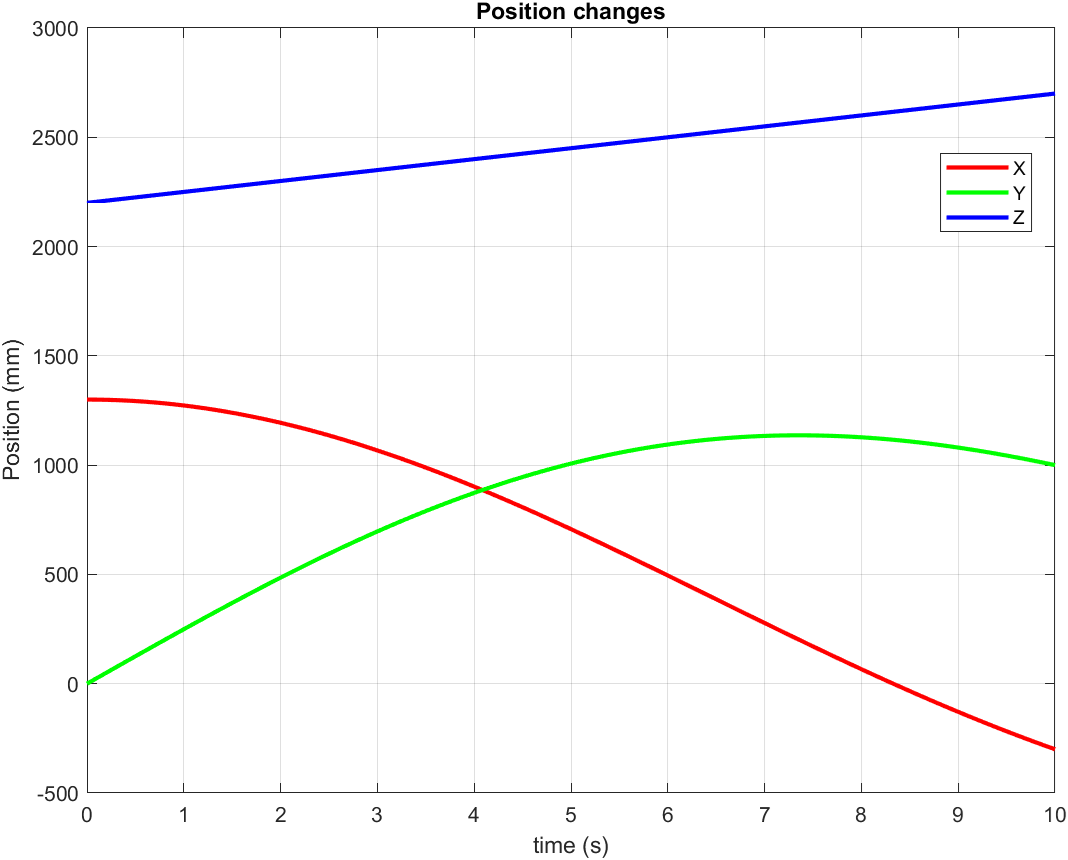
\includegraphics[width=0.8\textwidth]{pictures/test_forward.png}
    \caption{The position of the end-effector $(x,y,z)$ with respect to time}
    \label{fig:forward_kinematic}
\end{figure}
Solution check:
\begin{itemize}
    \item At time \( t = 0 \) s, the end-effector is at position \( (x,y,z) = (1300,0,2200) \) mm. Correct!\\
    \item At time \( t = 10 \) s, the end-effector is at position \( (x,y,z) = (-300,1000,2700) \) mm. Correct!\\
\end{itemize}
So we can confirm the accurate of the solution.
% check the forward kinematic problem with the following values: